%%%\documentclass{article}
%%%\usepackage[x11names, rgb]{xcolor}
%%%\usepackage{tikz}
%%%\usetikzlibrary{decorations,arrows,shapes}
%%%\begin{document}
%%%\fbox{
%%%

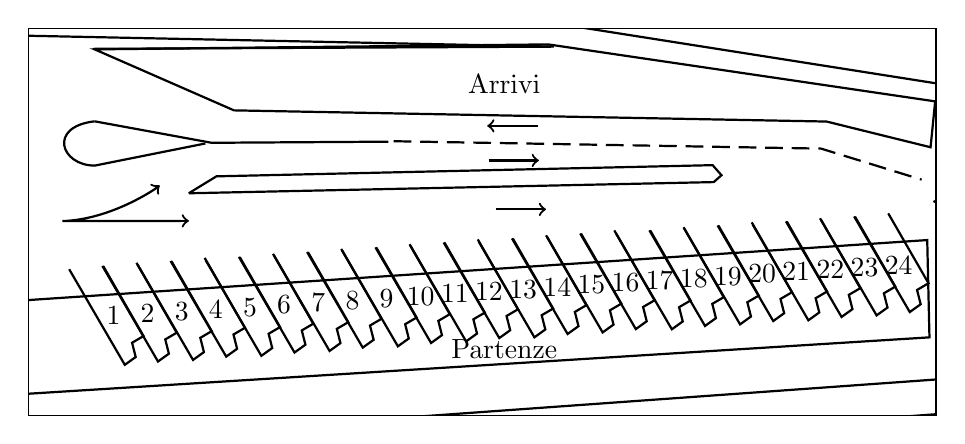
\begin{tikzpicture}[y=0.80pt,x=0.80pt,yscale=-1, inner sep=0pt, outer sep=0pt,scale=0.5]
\begin{scope}% layer1

\draw[clip] (100,280)--++(820,0)--++(0,350)--++(-820,0)--cycle;

  % linea_bassa
  \path[draw=black,line join=miter,line cap=butt,line width=0.800pt]
    (441.3734,664.2890) -- (1032.5857,620.3145);

  % linea_confine_basso
  \path[draw=black,line join=miter,line cap=butt,line width=0.800pt]
    (53.7466,659.4029) -- (1030.9570,589.3695);

  % tettoia_arrivi
  \path[draw=black,line join=miter,line cap=butt,line width=0.800pt]
    (1029.2929,362.2763) -- (569.6970,294.5995) -- (160.0000,299.0945) --
    (285.8586,354.1955) -- (821.2121,364.2965) -- (915.1515,387.5288) --
    (919.1919,347.1248);

  % marciapiede_centrale
  \path[draw=black,line join=miter,line cap=butt,line width=0.796pt]
    (245.0000,429.0945) -- (270.0136,413.7915) -- (718.2583,403.6904) --
    (726.2626,412.7814) -- (719.2588,418.9935) -- (245.0000,429.0945);

  % divisore_centrale
  \path[draw=black,line join=miter,line cap=butt,line width=0.800pt]
    (425.2525,382.4783) -- (265.6566,383.4884) -- (160.0000,364.0945);

  % perimetro_esterno_alto
  \path[draw=black,line join=miter,line cap=butt,line width=0.800pt]
    (1030.3030,347.1248) -- (574.7475,275.4076) -- (36.5862,260.9196);

  % perimetro_interno_e_tettoia_partenze
  \path[draw=black,line join=miter,line cap=butt,line width=0.800pt]
    (158.5859,298.6399) -- (574.7475,296.6197) -- (38.3838,285.5086) --
    (38.3838,611.7713) -- (74.7475,611.7713) -- (914.1414,559.2460) --
    (912.1212,471.3672) -- (64.6465,527.9329) -- (71.7172,612.7813);

  % rotonda_interna
  \path[draw=black,line join=miter,line cap=butt,line width=0.800pt]
    (160.0000,364.0945) .. controls (117.6512,368.9171) and (129.1846,403.9173) ..
    (160.0000,404.0945) -- (260.0000,384.0945);

% partenze
\draw[] (530, 570) node {Partenze};
% arrivi
\draw[] (530, 330) node {Arrivi};
% numero piattaforma
\foreach \p/\x/\y in {1/177/540, 2/207.84/538, 3/238.68/536, 4/269.52/534, 5/300.36/532, 6/331.2/530,
 7/362.04/528, 8/392.88/526, 9/423.72/524, 10/454.56/522, 11/485.4/520, 12/516.2
4/518, 13/547.08/516, 14/577.92/514, 15/608.76/512, 16/639.6/510, 17/670.44/508,
 18/701.28/506, 19/732.12/504, 20/762.96/502, 21/793.8/500, 22/824.64/498, 23/85
5.48/496, 24/886.32/494}
{
	\draw[] (\x, \y)  node {\p};
}

  % piattaforma_01
  \path[draw=black,line join=miter,line cap=butt,line width=0.800pt]
    (167.8025,494.9317) -- (204.1661,558.0630) -- (193.8126,564.1236) --
    (197.0954,577.0024) -- (187.2470,584.0731) -- (136.9944,497.7095);

  % piattaforma_02
  \path[draw=black,line join=miter,line cap=butt,line width=0.800pt]
    (197.7722,491.9266) -- (234.1358,555.0580) -- (223.7823,561.1186) --
    (227.0651,573.9973) -- (217.2166,581.0680) -- (166.9641,494.7044);

  % piattaforma_03
  \path[draw=black,line join=miter,line cap=butt,line width=0.800pt]
    (229.4341,490.4989) -- (265.7978,553.6302) -- (255.4442,559.6908) --
    (258.7271,572.5696) -- (248.8786,579.6403) -- (198.6261,493.2766);

  % piattaforma_04
  \path[draw=black,line join=miter,line cap=butt,line width=0.800pt]
    (259.4038,487.4938) -- (295.7674,550.6251) -- (285.4139,556.6857) --
    (288.6967,569.5645) -- (278.8483,576.6352) -- (228.5958,490.2716);

  % piattaforma_05
  \path[draw=black,line join=miter,line cap=butt,line width=0.800pt]
    (291.1427,486.8126) -- (327.5063,549.9439) -- (317.1528,556.0046) --
    (320.4356,568.8833) -- (310.5871,575.9540) -- (260.3346,489.5904);

  % piattaforma_06
  \path[draw=black,line join=miter,line cap=butt,line width=0.800pt]
    (321.1124,483.8076) -- (357.4760,546.9389) -- (347.1225,552.9995) --
    (350.4053,565.8783) -- (340.5568,572.9490) -- (290.3043,486.5854);

  % piattaforma_07
  \path[draw=black,line join=miter,line cap=butt,line width=0.800pt]
    (352.7743,482.3798) -- (389.1379,545.5111) -- (378.7844,551.5717) --
    (382.0672,564.4505) -- (372.2188,571.5212) -- (321.9662,485.1576);

  % piattaforma_08
  \path[draw=black,line join=miter,line cap=butt,line width=0.800pt]
    (382.7440,479.3748) -- (419.1076,542.5061) -- (408.7541,548.5667) --
    (412.0369,561.4455) -- (402.1884,568.5162) -- (351.9359,482.1525);

  % piattaforma_09
  \path[draw=black,line join=miter,line cap=butt,line width=0.800pt]
    (414.4888,478.1939) -- (450.8524,541.3252) -- (440.4989,547.3859) --
    (443.7817,560.2646) -- (433.9332,567.3353) -- (383.6807,480.9717);

  % piattaforma_10
  \path[draw=black,line join=miter,line cap=butt,line width=0.800pt]
    (444.4585,475.1889) -- (480.8221,538.3202) -- (470.4686,544.3808) --
    (473.7514,557.2596) -- (463.9029,564.3303) -- (413.6504,477.9667);

  % piattaforma_11
  \path[draw=black,line join=miter,line cap=butt,line width=0.800pt]
    (476.1204,473.7611) -- (512.4841,536.8924) -- (502.1305,542.9530) --
    (505.4134,555.8318) -- (495.5649,562.9025) -- (445.3123,476.5389);

  % piattaforma_12
  \path[draw=black,line join=miter,line cap=butt,line width=0.800pt]
    (506.0901,470.7561) -- (542.4537,533.8874) -- (532.1002,539.9480) --
    (535.3830,552.8268) -- (525.5346,559.8975) -- (475.2820,473.5338);

  % piattaforma_13
  \path[draw=black,line join=miter,line cap=butt,line width=0.800pt]
    (537.8290,470.0749) -- (574.1926,533.2062) -- (563.8391,539.2668) --
    (567.1219,552.1456) -- (557.2734,559.2163) -- (507.0209,472.8527);

  % piattaforma_14
  \path[draw=black,line join=miter,line cap=butt,line width=0.800pt]
    (567.7986,467.0698) -- (604.1623,530.2011) -- (593.8088,536.2618) --
    (597.0916,549.1405) -- (587.2431,556.2112) -- (536.9906,469.8476);

  % piattaforma_15
  \path[draw=black,line join=miter,line cap=butt,line width=0.800pt]
    (599.4606,465.6421) -- (635.8242,528.7734) -- (625.4707,534.8340) --
    (628.7535,547.7128) -- (618.9051,554.7835) -- (568.6525,468.4198);

  % piattaforma_16
  \path[draw=black,line join=miter,line cap=butt,line width=0.800pt]
    (629.4303,462.6370) -- (665.7939,525.7683) -- (655.4404,531.8289) --
    (658.7232,544.7077) -- (648.8747,551.7784) -- (598.6222,465.4148);

  % piattaforma_17
  \path[draw=black,line join=miter,line cap=butt,line width=0.800pt]
    (661.9724,462.8104) -- (698.3361,525.9417) -- (687.9826,532.0023) --
    (691.2654,544.8811) -- (681.4169,551.9518) -- (631.1644,465.5882);

  % piattaforma_18
  \path[draw=black,line join=miter,line cap=butt,line width=0.800pt]
    (691.9421,459.8054) -- (728.3058,522.9367) -- (717.9522,528.9973) --
    (721.2351,541.8761) -- (711.3866,548.9468) -- (661.1341,462.5831);

  % piattaforma_19
  \path[draw=black,line join=miter,line cap=butt,line width=0.800pt]
    (723.6041,458.3776) -- (759.9677,521.5089) -- (749.6142,527.5695) --
    (752.8970,540.4483) -- (743.0485,547.5190) -- (692.7960,461.1554);

  % piattaforma_20
  \path[draw=black,line join=miter,line cap=butt,line width=0.800pt]
    (753.5738,455.3725) -- (789.9374,518.5039) -- (779.5839,524.5645) --
    (782.8667,537.4432) -- (773.0182,544.5140) -- (722.7657,458.1503);

  % piattaforma_21
  \path[draw=black,line join=miter,line cap=butt,line width=0.800pt]
    (785.3126,454.6914) -- (821.6763,517.8227) -- (811.3227,523.8833) --
    (814.6056,536.7621) -- (804.7571,543.8328) -- (754.5045,457.4691);

  % piattaforma_22
  \path[draw=black,line join=miter,line cap=butt,line width=0.800pt]
    (815.2823,451.6863) -- (851.6460,514.8176) -- (841.2924,520.8782) --
    (844.5752,533.7570) -- (834.7268,540.8277) -- (784.4742,454.4641);

  % piattaforma_23
  \path[draw=black,line join=miter,line cap=butt,line width=0.800pt]
    (846.9443,450.2585) -- (883.3079,513.3899) -- (872.9544,519.4505) --
    (876.2372,532.3292) -- (866.3887,539.3999) -- (816.1362,453.0363);

  % piattaforma_24
  \path[draw=black,line join=miter,line cap=butt,line width=0.800pt]
    (876.9140,447.2535) -- (913.2776,510.3848) -- (902.9241,516.4454) --
    (906.2069,529.3242) -- (896.3584,536.3949) -- (846.1059,450.0313);

  % segnaletica
  \path[draw=black,dash pattern=on 6.39pt off 3.20pt,line join=miter,line
    cap=butt,miter limit=4.00,line width=0.799pt] (430.1588,382.0665) --
    (816.2329,388.7459) -- (907.0739,416.7998);

  % freccia_sx_entrata
  \path[draw=black,line join=miter,line cap=butt,line width=0.800pt,->]
    (960.5098,415.4639) -- (923.1047,395.4254);

  % freccia_dx_centrale
  \path[draw=black,line join=miter,line cap=butt,line width=0.800pt,->]
    (515.8896,399.4331) -- (561.3101,399.4331);

  % freccia_dx_uscita
  \path[draw=black,line join=miter,line cap=butt,line width=0.800pt,->]
    (917.7611,436.1011) -- (955.1662,456.1395);

  % rotonda_ingresso
  \path[shift={(28.0,32.0)},draw=black,dash pattern=on 6.39pt off 3.20pt,line
    join=miter,miter limit=4.00,line width=0.799pt]
    (1020.6251,444.8536)arc(0.000:180.000:22.710)arc(-180.000:0.000:22.710) --
    cycle;

  % freccia_sx_arrivi
  \path[draw=black,line join=miter,line cap=butt,line width=0.800pt,->]
     (560.0818,368.1895) -- (514.6614,368.1895);

  % diramazione
  \path[draw=black,line join=miter,line cap=butt,line width=0.800pt,->]
    (237.7896,454.2049) -- (130.9179,454.2049) .. controls (175.0025,452.8690) and
    (215.0794,424.8152) .. (215.0794,424.8152) -- (218.7531,421.9764);

  % freccia_dx_diramazione
  \path[draw=black,line join=miter,line cap=butt,line width=0.800pt,->]
    (237.6226,454.0379) -- (245.1371,454.0379);

  % freccia_dx_partenze
  \path[draw=black,line join=miter,line cap=butt,line width=0.800pt,->]
    (522.3356,443.6177) -- (567.7561,443.6177);

\end{scope}

\end{tikzpicture}

%%%
%%%}
%%%\end{document}

